% IPTV quick start guide, English edition. Build in this folder with:
%   pdflatex IPTV-Quick-Start.tex   (run it twice, for the table of contents)
% Other languages: IPTV-Quick-Start-it.tex, -es, -fr, -de, -pt (same layout,
% from preamble.tex).
\newcommand{\GuideLang}{english}
\newcommand{\GuideTitle}{Quick Start Guide}
\newcommand{\TipLabel}{Tip.}
% Shared layout of the IPTV quick start guides (one file per language:
% IPTV-Quick-Start.tex, IPTV-Quick-Start-it.tex, ...). Each sets, before
% % Shared layout of the IPTV quick start guides (one file per language:
% IPTV-Quick-Start.tex, IPTV-Quick-Start-it.tex, ...). Each sets, before
% % Shared layout of the IPTV quick start guides (one file per language:
% IPTV-Quick-Start.tex, IPTV-Quick-Start-it.tex, ...). Each sets, before
% \input{preamble}:
%   \GuideLang   babel language (english, italian, spanish, french, ngerman, portuguese)
%   \GuideTitle  the guide's title, used on the cover, in headers and the PDF
%   \TipLabel    the word that starts a tip box ("Tip.")
% Build any of them with pdflatex, twice (for the table of contents).
\documentclass[11pt,a4paper]{article}

\usepackage[T1]{fontenc}
\usepackage[utf8]{inputenc}
% shorthands=off: no language-specific active characters (they would clash
% with tables and addresses); only hyphenation and "Contents" etc. change.
\usepackage[shorthands=off,\GuideLang]{babel}
\usepackage{lmodern}
\usepackage[scaled=0.92]{helvet}
\renewcommand{\familydefault}{\sfdefault}
\usepackage[margin=2.2cm,headheight=14pt]{geometry}
\usepackage{graphicx}
\usepackage[table]{xcolor}
\usepackage{booktabs}
\usepackage{tabularx}
\usepackage{xltabular}
\usepackage{enumitem}
\usepackage{titlesec}
\usepackage{fancyhdr}
\usepackage{pifont}
\usepackage{amssymb}
\usepackage[hidelinks]{hyperref}

\newcommand{\version}{0.12}
\definecolor{accent}{HTML}{1E6FD9}
\definecolor{dim}{HTML}{5F6673}
\definecolor{notebg}{HTML}{EEF4FC}
\definecolor{warnbg}{HTML}{FFF6E0}
\definecolor{tvred}{HTML}{D32F2F}
\definecolor{tvgreen}{HTML}{2E7D32}
\definecolor{tvyellow}{HTML}{C9A400}
\definecolor{tvblue}{HTML}{1565C0}

\hypersetup{pdftitle={IPTV -- \GuideTitle}, pdfauthor={IPTV project}}
\setlist{itemsep=2pt, topsep=4pt}
\setlength{\parindent}{0pt}
\setlength{\parskip}{6pt}
\renewcommand{\arraystretch}{1.25}

\titleformat{\section}{\Large\bfseries\color{accent}}{\thesection}{0.6em}{}
\titleformat{\subsection}{\large\bfseries}{\thesubsection}{0.6em}{}
\titlespacing*{\section}{0pt}{14pt}{6pt}
\titlespacing*{\subsection}{0pt}{10pt}{4pt}

\pagestyle{fancy}
\fancyhf{}
\fancyhead[L]{\small\color{dim}IPTV -- \GuideTitle}
\fancyhead[R]{\small\color{dim}github.com/vickdini/iptv}
\fancyfoot[C]{\small\color{dim}\thepage}
\renewcommand{\headrulewidth}{0.4pt}
\renewcommand{\sectionmark}[1]{\markboth{#1}{}}

% A key or button on a keyboard / remote.
\newcommand{\key}[1]{{\setlength{\fboxsep}{1.5pt}\fbox{\footnotesize\vphantom{Ay}#1}}}
% A coloured remote button.
\newcommand{\colorkey}[2]{\textcolor{#1}{\ding{108}}\,\textbf{#2}}
% Shaded boxes for tips and notes.
\newcommand{\tip}[1]{\par\noindent\colorbox{notebg}{\parbox{\dimexpr\linewidth-2\fboxsep}{\small\textbf{\TipLabel} #1}}\par}
\newcommand{\note}[1]{\par\noindent\colorbox{warnbg}{\parbox{\dimexpr\linewidth-2\fboxsep}{\small #1}}\par}
\newcommand{\menu}[1]{\textit{#1}}
\newcommand{\download}{\url{https://github.com/vickdini/iptv/releases/latest}}
% Key tables: \rowcolors{2}{gray!8}{white} then
% \begin{xltabular}{\linewidth}{@{}KX@{}} \keyshead{Key}{What it does} ... \bottomrule
\newcolumntype{K}{>{\raggedright\arraybackslash}p{5.4cm}}
\newcommand{\keyshead}[2]{\toprule \textbf{#1} & \textbf{#2} \\ \midrule}

% The cover: #1 subtitle, #2 "Version".
\newcommand{\cover}[2]{%
\begin{titlepage}
  \centering
  \vspace*{0.5cm}
  {\fontsize{40}{48}\selectfont\bfseries\color{accent} IPTV\par}
  \vspace{0.3cm}
  {\LARGE \GuideTitle\par}
  \vspace{0.3cm}
  {\large\color{dim} #1\par}
  \vspace{1cm}
  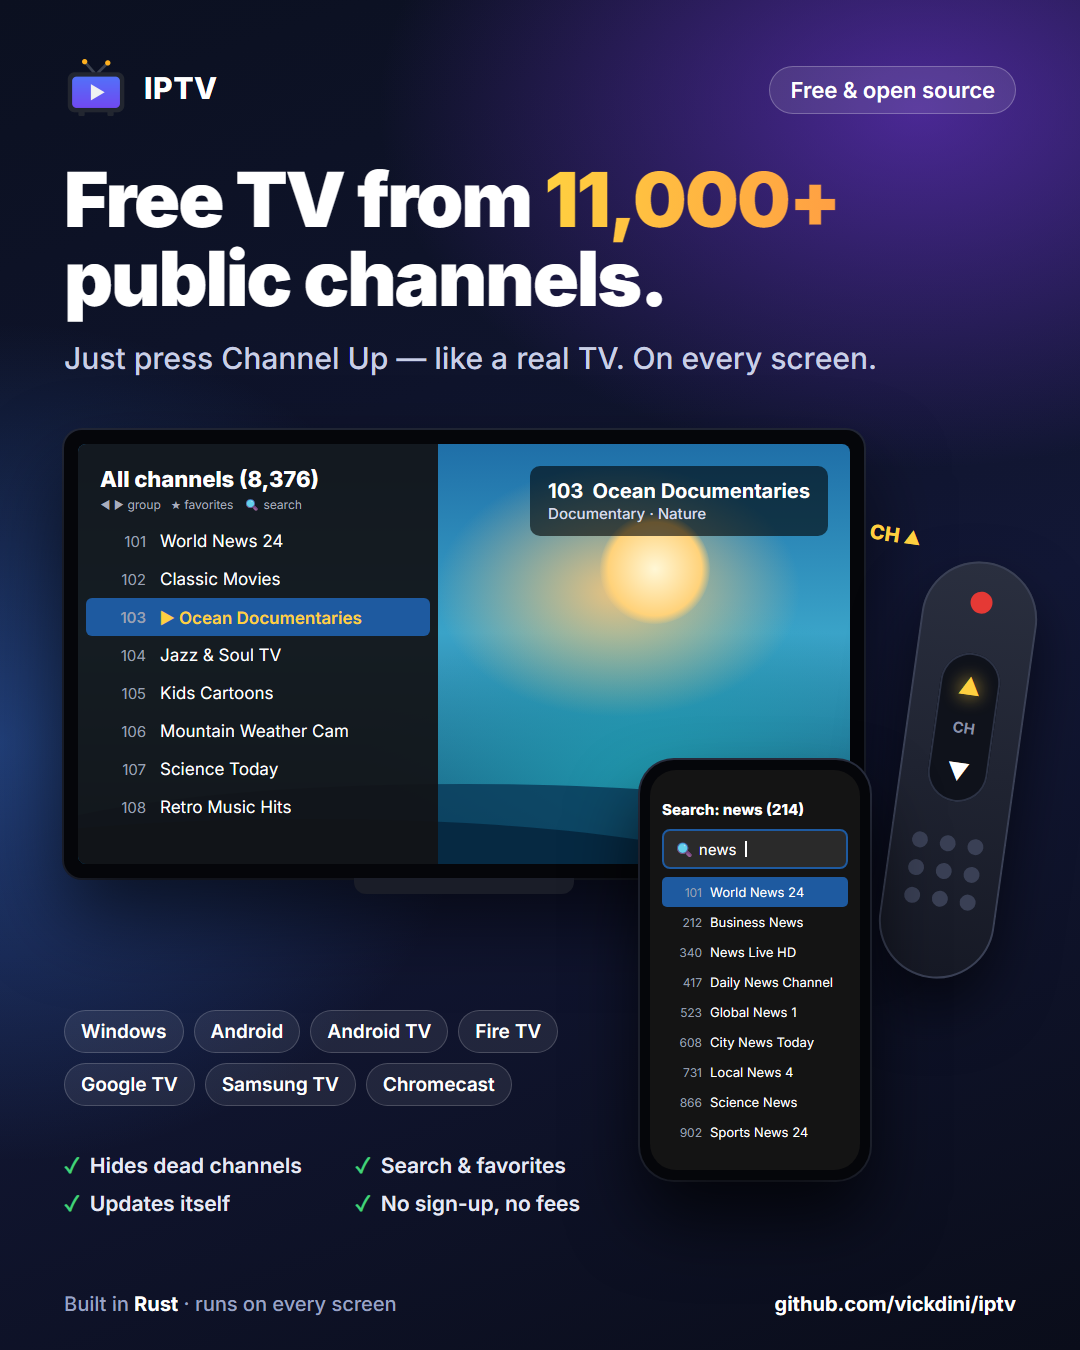
\includegraphics[width=0.52\textwidth]{../images/iptv-overview.png}\par
  \vfill
  {\large Windows \textbullet{} macOS \textbullet{} Linux \textbullet{} Android
   \textbullet{} Android TV \& Fire TV \textbullet{} Chromecast \textbullet{} Samsung TV\par}
  \vspace{0.5cm}
  {\color{dim} #2 \version{} \textbullet{} \url{https://github.com/vickdini/iptv}\par}
\end{titlepage}
\tableofcontents
\thispagestyle{fancy}}
:
%   \GuideLang   babel language (english, italian, spanish, french, ngerman, portuguese)
%   \GuideTitle  the guide's title, used on the cover, in headers and the PDF
%   \TipLabel    the word that starts a tip box ("Tip.")
% Build any of them with pdflatex, twice (for the table of contents).
\documentclass[11pt,a4paper]{article}

\usepackage[T1]{fontenc}
\usepackage[utf8]{inputenc}
% shorthands=off: no language-specific active characters (they would clash
% with tables and addresses); only hyphenation and "Contents" etc. change.
\usepackage[shorthands=off,\GuideLang]{babel}
\usepackage{lmodern}
\usepackage[scaled=0.92]{helvet}
\renewcommand{\familydefault}{\sfdefault}
\usepackage[margin=2.2cm,headheight=14pt]{geometry}
\usepackage{graphicx}
\usepackage[table]{xcolor}
\usepackage{booktabs}
\usepackage{tabularx}
\usepackage{xltabular}
\usepackage{enumitem}
\usepackage{titlesec}
\usepackage{fancyhdr}
\usepackage{pifont}
\usepackage{amssymb}
\usepackage[hidelinks]{hyperref}

\newcommand{\version}{0.12}
\definecolor{accent}{HTML}{1E6FD9}
\definecolor{dim}{HTML}{5F6673}
\definecolor{notebg}{HTML}{EEF4FC}
\definecolor{warnbg}{HTML}{FFF6E0}
\definecolor{tvred}{HTML}{D32F2F}
\definecolor{tvgreen}{HTML}{2E7D32}
\definecolor{tvyellow}{HTML}{C9A400}
\definecolor{tvblue}{HTML}{1565C0}

\hypersetup{pdftitle={IPTV -- \GuideTitle}, pdfauthor={IPTV project}}
\setlist{itemsep=2pt, topsep=4pt}
\setlength{\parindent}{0pt}
\setlength{\parskip}{6pt}
\renewcommand{\arraystretch}{1.25}

\titleformat{\section}{\Large\bfseries\color{accent}}{\thesection}{0.6em}{}
\titleformat{\subsection}{\large\bfseries}{\thesubsection}{0.6em}{}
\titlespacing*{\section}{0pt}{14pt}{6pt}
\titlespacing*{\subsection}{0pt}{10pt}{4pt}

\pagestyle{fancy}
\fancyhf{}
\fancyhead[L]{\small\color{dim}IPTV -- \GuideTitle}
\fancyhead[R]{\small\color{dim}github.com/vickdini/iptv}
\fancyfoot[C]{\small\color{dim}\thepage}
\renewcommand{\headrulewidth}{0.4pt}
\renewcommand{\sectionmark}[1]{\markboth{#1}{}}

% A key or button on a keyboard / remote.
\newcommand{\key}[1]{{\setlength{\fboxsep}{1.5pt}\fbox{\footnotesize\vphantom{Ay}#1}}}
% A coloured remote button.
\newcommand{\colorkey}[2]{\textcolor{#1}{\ding{108}}\,\textbf{#2}}
% Shaded boxes for tips and notes.
\newcommand{\tip}[1]{\par\noindent\colorbox{notebg}{\parbox{\dimexpr\linewidth-2\fboxsep}{\small\textbf{\TipLabel} #1}}\par}
\newcommand{\note}[1]{\par\noindent\colorbox{warnbg}{\parbox{\dimexpr\linewidth-2\fboxsep}{\small #1}}\par}
\newcommand{\menu}[1]{\textit{#1}}
\newcommand{\download}{\url{https://github.com/vickdini/iptv/releases/latest}}
% Key tables: \rowcolors{2}{gray!8}{white} then
% \begin{xltabular}{\linewidth}{@{}KX@{}} \keyshead{Key}{What it does} ... \bottomrule
\newcolumntype{K}{>{\raggedright\arraybackslash}p{5.4cm}}
\newcommand{\keyshead}[2]{\toprule \textbf{#1} & \textbf{#2} \\ \midrule}

% The cover: #1 subtitle, #2 "Version".
\newcommand{\cover}[2]{%
\begin{titlepage}
  \centering
  \vspace*{0.5cm}
  {\fontsize{40}{48}\selectfont\bfseries\color{accent} IPTV\par}
  \vspace{0.3cm}
  {\LARGE \GuideTitle\par}
  \vspace{0.3cm}
  {\large\color{dim} #1\par}
  \vspace{1cm}
  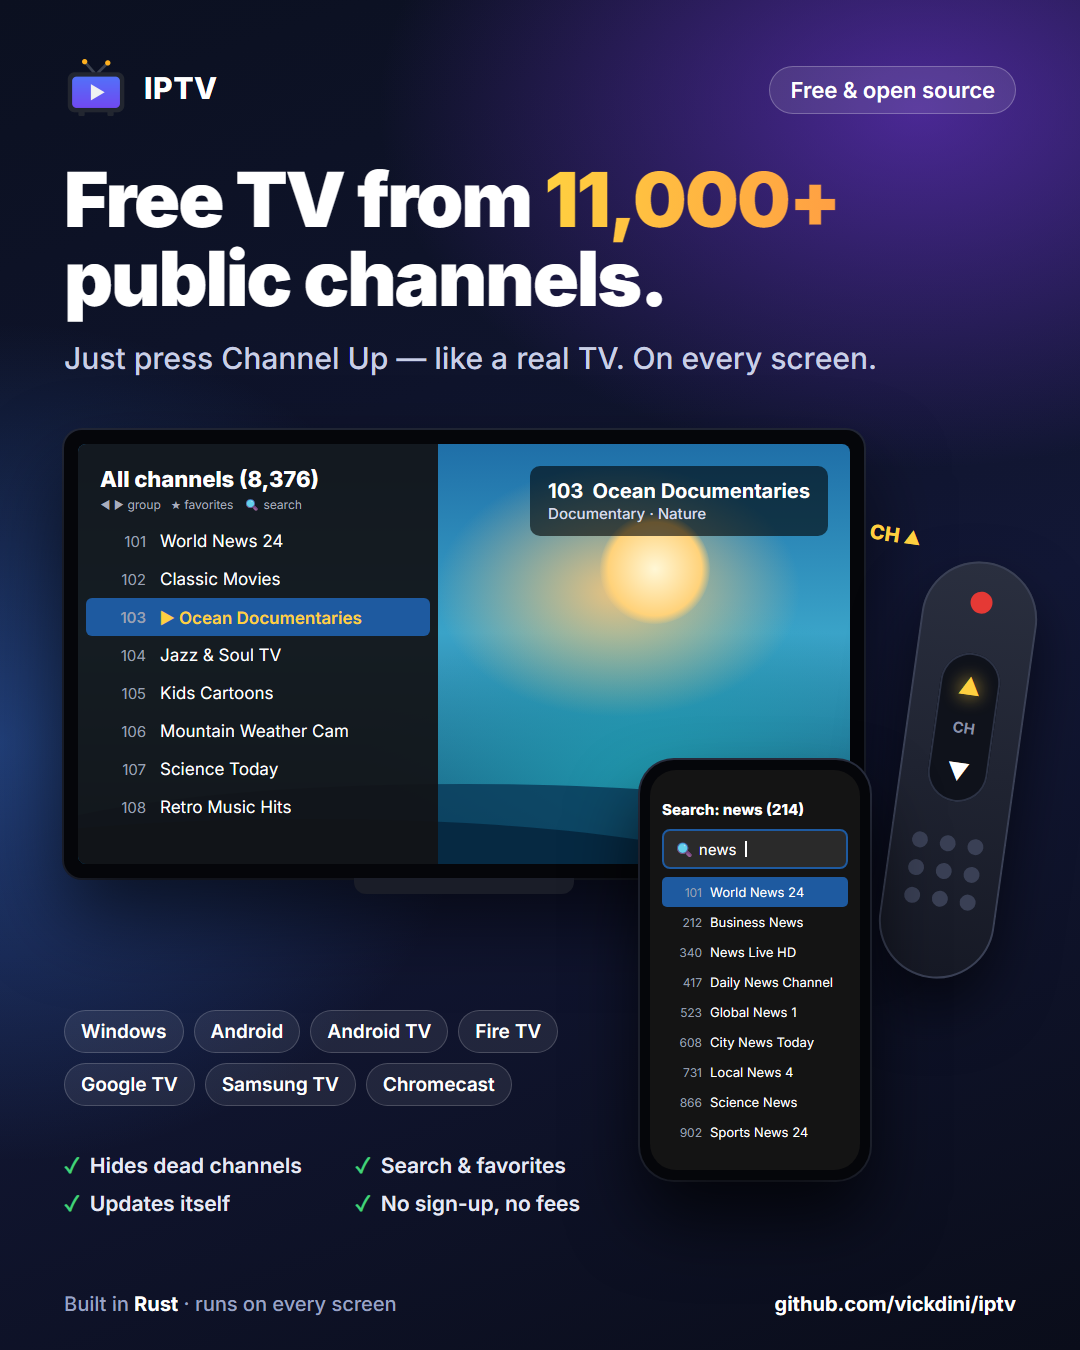
\includegraphics[width=0.52\textwidth]{../images/iptv-overview.png}\par
  \vfill
  {\large Windows \textbullet{} macOS \textbullet{} Linux \textbullet{} Android
   \textbullet{} Android TV \& Fire TV \textbullet{} Chromecast \textbullet{} Samsung TV\par}
  \vspace{0.5cm}
  {\color{dim} #2 \version{} \textbullet{} \url{https://github.com/vickdini/iptv}\par}
\end{titlepage}
\tableofcontents
\thispagestyle{fancy}}
:
%   \GuideLang   babel language (english, italian, spanish, french, ngerman, portuguese)
%   \GuideTitle  the guide's title, used on the cover, in headers and the PDF
%   \TipLabel    the word that starts a tip box ("Tip.")
% Build any of them with pdflatex, twice (for the table of contents).
\documentclass[11pt,a4paper]{article}

\usepackage[T1]{fontenc}
\usepackage[utf8]{inputenc}
% shorthands=off: no language-specific active characters (they would clash
% with tables and addresses); only hyphenation and "Contents" etc. change.
\usepackage[shorthands=off,\GuideLang]{babel}
\usepackage{lmodern}
\usepackage[scaled=0.92]{helvet}
\renewcommand{\familydefault}{\sfdefault}
\usepackage[margin=2.2cm,headheight=14pt]{geometry}
\usepackage{graphicx}
\usepackage[table]{xcolor}
\usepackage{booktabs}
\usepackage{tabularx}
\usepackage{xltabular}
\usepackage{enumitem}
\usepackage{titlesec}
\usepackage{fancyhdr}
\usepackage{pifont}
\usepackage{amssymb}
\usepackage[hidelinks]{hyperref}

\newcommand{\version}{0.12}
\definecolor{accent}{HTML}{1E6FD9}
\definecolor{dim}{HTML}{5F6673}
\definecolor{notebg}{HTML}{EEF4FC}
\definecolor{warnbg}{HTML}{FFF6E0}
\definecolor{tvred}{HTML}{D32F2F}
\definecolor{tvgreen}{HTML}{2E7D32}
\definecolor{tvyellow}{HTML}{C9A400}
\definecolor{tvblue}{HTML}{1565C0}

\hypersetup{pdftitle={IPTV -- \GuideTitle}, pdfauthor={IPTV project}}
\setlist{itemsep=2pt, topsep=4pt}
\setlength{\parindent}{0pt}
\setlength{\parskip}{6pt}
\renewcommand{\arraystretch}{1.25}

\titleformat{\section}{\Large\bfseries\color{accent}}{\thesection}{0.6em}{}
\titleformat{\subsection}{\large\bfseries}{\thesubsection}{0.6em}{}
\titlespacing*{\section}{0pt}{14pt}{6pt}
\titlespacing*{\subsection}{0pt}{10pt}{4pt}

\pagestyle{fancy}
\fancyhf{}
\fancyhead[L]{\small\color{dim}IPTV -- \GuideTitle}
\fancyhead[R]{\small\color{dim}github.com/vickdini/iptv}
\fancyfoot[C]{\small\color{dim}\thepage}
\renewcommand{\headrulewidth}{0.4pt}
\renewcommand{\sectionmark}[1]{\markboth{#1}{}}

% A key or button on a keyboard / remote.
\newcommand{\key}[1]{{\setlength{\fboxsep}{1.5pt}\fbox{\footnotesize\vphantom{Ay}#1}}}
% A coloured remote button.
\newcommand{\colorkey}[2]{\textcolor{#1}{\ding{108}}\,\textbf{#2}}
% Shaded boxes for tips and notes.
\newcommand{\tip}[1]{\par\noindent\colorbox{notebg}{\parbox{\dimexpr\linewidth-2\fboxsep}{\small\textbf{\TipLabel} #1}}\par}
\newcommand{\note}[1]{\par\noindent\colorbox{warnbg}{\parbox{\dimexpr\linewidth-2\fboxsep}{\small #1}}\par}
\newcommand{\menu}[1]{\textit{#1}}
\newcommand{\download}{\url{https://github.com/vickdini/iptv/releases/latest}}
% Key tables: \rowcolors{2}{gray!8}{white} then
% \begin{xltabular}{\linewidth}{@{}KX@{}} \keyshead{Key}{What it does} ... \bottomrule
\newcolumntype{K}{>{\raggedright\arraybackslash}p{5.4cm}}
\newcommand{\keyshead}[2]{\toprule \textbf{#1} & \textbf{#2} \\ \midrule}

% The cover: #1 subtitle, #2 "Version".
\newcommand{\cover}[2]{%
\begin{titlepage}
  \centering
  \vspace*{0.5cm}
  {\fontsize{40}{48}\selectfont\bfseries\color{accent} IPTV\par}
  \vspace{0.3cm}
  {\LARGE \GuideTitle\par}
  \vspace{0.3cm}
  {\large\color{dim} #1\par}
  \vspace{1cm}
  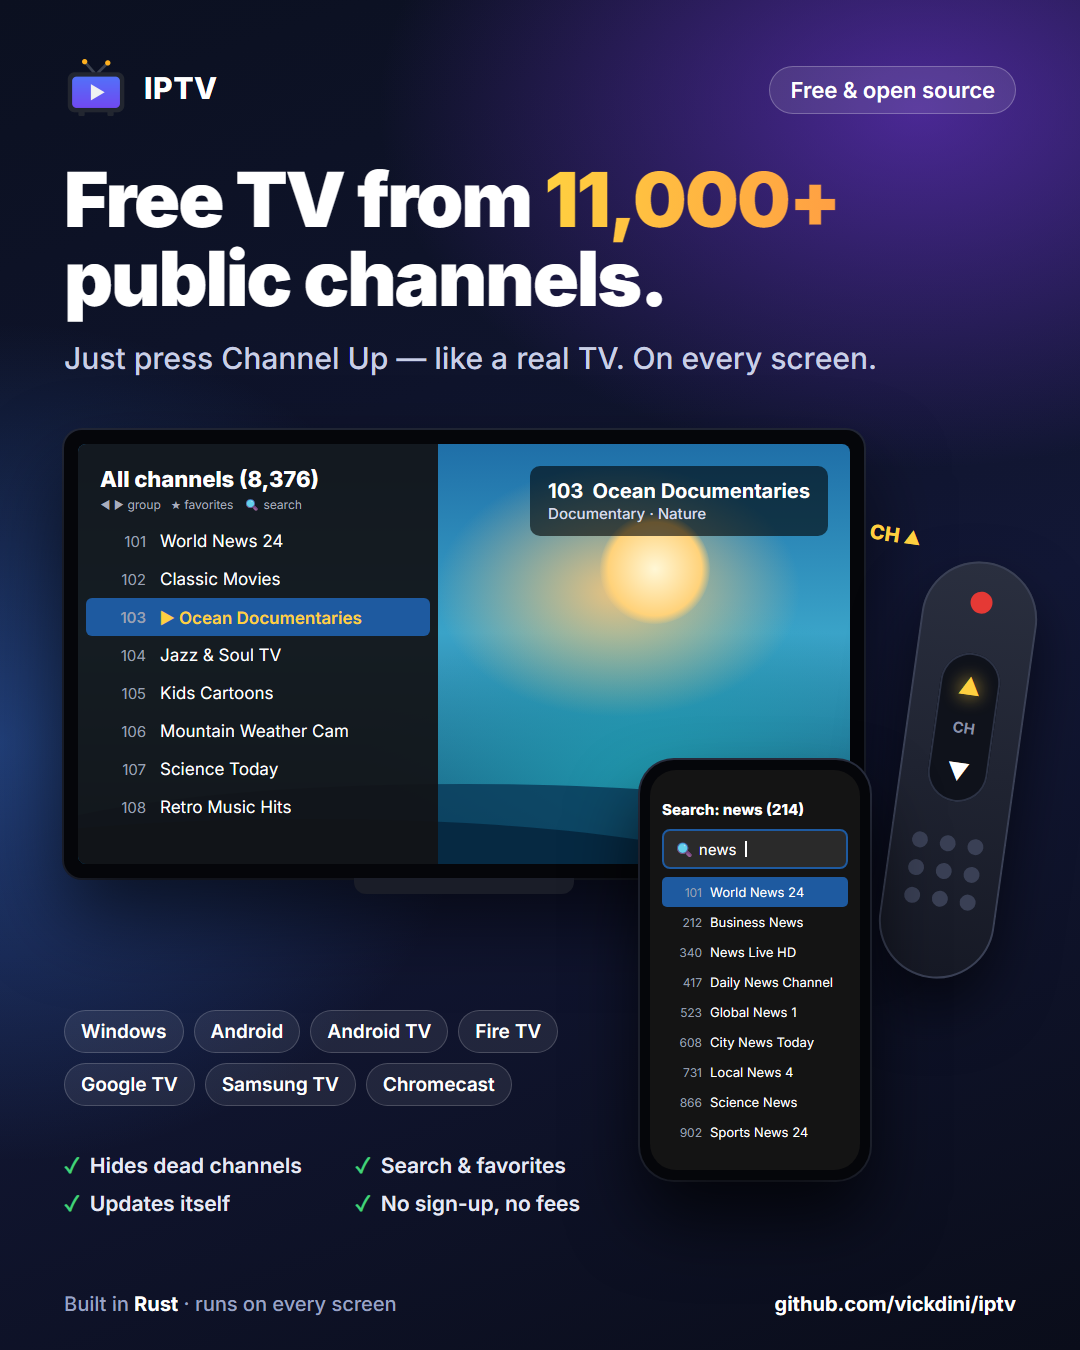
\includegraphics[width=0.52\textwidth]{../images/iptv-overview.png}\par
  \vfill
  {\large Windows \textbullet{} macOS \textbullet{} Linux \textbullet{} Android
   \textbullet{} Android TV \& Fire TV \textbullet{} Chromecast \textbullet{} Samsung TV\par}
  \vspace{0.5cm}
  {\color{dim} #2 \version{} \textbullet{} \url{https://github.com/vickdini/iptv}\par}
\end{titlepage}
\tableofcontents
\thispagestyle{fancy}}


\begin{document}
\cover{Watch free TV channels and zap like a TV}{Version}

% ------------------------------------------------------------------ intro
\section{About IPTV}

IPTV plays the free, publicly listed TV channels collected by the
\emph{iptv-org} project (more than 10\,000 of them) and lets you switch
between them like on a television: channel up and down, channel numbers,
favorites and groups such as News, Movies or Sports.

\begin{itemize}
  \item \textbf{Always up to date.} The channel list is refreshed each time
        IPTV starts, and the app updates itself when a new version is out.
  \item \textbf{Only channels that work.} Offline channels are hidden
        automatically, so zapping never stops on a black screen.
  \item \textbf{Find channels quickly.} Search by name, see each channel's
        logo, go back to the channels you watched recently, or show only the
        countries and languages you are interested in.
  \item \textbf{Your language.} IPTV speaks English, Italian, Spanish,
        French, German and Portuguese, and follows your device's language.
        On channels that broadcast it, choose the audio language and turn on
        subtitles.
  \item \textbf{Phone remote.} Control the TV or computer from your phone's
        browser (Section~\ref{sec:remote}).
\end{itemize}

Everything you need is included in each download: there is nothing else to
install. All downloads are on the release page:

\begin{center}
  \download
\end{center}

\note{\textbf{Disclaimer.} IPTV doesn't host or provide any video: it only
loads a publicly available playlist published by the iptv-org project. Only
watch what you are legally allowed to watch in your country.}

% ------------------------------------------------------------------ Windows
\section{Windows}
\label{sec:windows}

\subsection{Install}
\begin{enumerate}
  \item Download \texttt{IPTV-Setup-\textless version\textgreater.exe} from
        the release page and open it.
  \item If Windows says \menu{Windows protected your PC}, click
        \menu{More info} and then \menu{Run anyway}.
  \item Follow the installer. It needs no administrator rights, and adds a
        Start-menu shortcut (and a desktop icon, if you want one).
\end{enumerate}
IPTV opens maximized and starts playing straight away. To remove it, use
\menu{Settings \textrightarrow{} Apps}.

\subsection{Keys}
\label{sec:keys}
These keys work on every computer: Windows, macOS and Linux.

\rowcolors{2}{gray!8}{white}
\begin{xltabular}{\linewidth}{@{}KX@{}}
\keyshead{Key}{What it does}
\key{$\uparrow$} \key{$\downarrow$}, \key{PgUp} \key{PgDn}, mouse wheel & next / previous channel \\
\key{0}--\key{9}, then wait or \key{Enter} & go to a channel number \\
\key{Backspace} & back to the previous channel \\
\key{$\leftarrow$} \key{$\rightarrow$}, \key{m} & volume down / up, mute \\
\key{l}, \key{Tab} or right-click & open / close the channel list \\
\key{/} or \key{Ctrl}+\key{F} & search channels by name \\
\key{c} & choose countries and languages \\
\key{g} / \key{G} & recently watched, then the groups (News, Movies\ldots) \\
\key{s} / \key{S} & add or remove a favorite / zap through favorites only \\
\key{a} / \key{t} & next audio language / next subtitles (and off) \\
\key{r} & phone remote: show the QR code \\
\key{E} / \key{I} & export / import favorites (Downloads folder) \\
\key{i} & channel information \\
\key{f}, double-click & full screen (\key{Esc} leaves it) \\
\key{p} & picture-in-picture: a second channel, small, in the bottom-right corner \\
\key{[} / \key{]} & the small picture's previous / next channel \\
\key{x}, click on the small picture & swap the two channels \\
\key{Space} & pause \\
\key{h}, \key{?} or \key{F1} & help on screen \\
\key{q} & quit \\
\bottomrule
\end{xltabular}

\subsection{The channel list}
Press \key{l} to open a scrollable list of channels, with their logos, on the
left; the video keeps playing beside it. Scroll with the mouse wheel and click
a channel to watch it. Start typing (or press \key{/}) to search: accents and
capital letters don't matter. \key{Esc} closes the list. Press \key{g} for the
channels you watched recently, most recent first.

\subsection{Countries and languages}
Press \key{c}, type to find a country or language, and press \key{Enter} to
tick it; \key{Tab} switches between the two lists. From then on IPTV shows
only channels from the ticked countries or in the ticked languages, until
you clear the choice (\key{Del}, or the \emph{Clear all} row).

\subsection{Audio language and subtitles}
When a channel offers more than one audio language or subtitles, a note at
the bottom of the screen says so. Press \key{a} for the next audio language
and \key{t} for the next subtitles (and finally \emph{off}). IPTV remembers
the language and uses it on every other channel that offers it.

\subsection{Language and updates}
IPTV uses the language of your system. Each time it starts, it checks for a
new version; if there is one, it installs it silently and restarts on its
own after a few seconds.

% ------------------------------------------------------------------ macOS
\section{macOS}

\subsection{Install}
\begin{enumerate}
  \item Find out which chip your Mac has: \menu{Apple menu \textrightarrow{}
        About This Mac}.
  \item Download the matching disk image from the release page:
  \begin{itemize}
    \item Apple silicon (M1, M2, M3, M4\ldots):
          \texttt{IPTV-\textless version\textgreater-macOS-arm64.dmg}
    \item Intel: \texttt{IPTV-\textless version\textgreater-macOS-x86\_64.dmg}
  \end{itemize}
  \item Open it and drag \textbf{IPTV} onto \textbf{Applications}.
\end{enumerate}

\subsection{First launch}
IPTV is not notarized by Apple, so the first time macOS refuses to open it.
This is needed only once:
\begin{enumerate}
  \item Open IPTV from Applications. When macOS says it can't be opened,
        click \menu{Done}.
  \item Open \menu{System Settings \textrightarrow{} Privacy \& Security},
        scroll down to \menu{``IPTV'' was blocked\ldots} and click
        \menu{Open Anyway}, then confirm.
\end{enumerate}

\subsection{Using it}
IPTV uses the same keys as on Windows (Section~\ref{sec:keys}). In the Dock
it appears as \textbf{IPTV} while a channel is playing.

\tip{Keep IPTV in the Applications folder: started from the disk image or
from Downloads, macOS runs it from a read-only copy and it can't update
itself.}

% ------------------------------------------------------------------ Linux
\section{Linux}

\subsection{Install}
Download \texttt{IPTV-\textless version\textgreater-x86\_64.AppImage} from the
release page. It is a single file with everything included. Make it
executable and run it:
\begin{center}
\begin{minipage}{0.8\linewidth}
\small\ttfamily chmod +x IPTV-*-x86\_64.AppImage\\
./IPTV-*-x86\_64.AppImage
\end{minipage}
\end{center}
In a file manager you can instead open \menu{Properties \textrightarrow{}
Permissions}, tick \menu{Allow executing as a program}, and double-click it.

It runs on 64-bit PCs with a Linux from 2022 or later (Ubuntu 22.04, Debian
12, Fedora 36, Linux Mint 21 and newer).

\tip{Tools such as \emph{Gear Lever} or \emph{AppImageLauncher} add IPTV to
the applications menu. If the AppImage complains that FUSE is missing, start
it with \texttt{-{}-appimage-extract-and-run}.}

\subsection{Using it}
IPTV uses the same keys as on Windows (Section~\ref{sec:keys}). It updates
itself by replacing the AppImage file, so keep it in a folder you can write
to (your home folder, for example).

% ------------------------------------------------------------------ Android
\section{Android phones and tablets}

\subsection{Install}
\begin{enumerate}
  \item On the phone, download \texttt{IPTV-\textless version\textgreater.apk}
        from the release page and open it.
  \item Android asks once to allow installing apps from your browser or file
        manager: allow it, then tap \menu{Install}.
  \item IPTV isn't on Google Play, so Play Protect may warn about an unknown
        developer: choose \menu{Install anyway}.
\end{enumerate}
You can also install it with \emph{Obtainium}, which keeps apps up to date
straight from their release page.

\subsection{Gestures}
\rowcolors{2}{gray!8}{white}
\begin{xltabular}{\linewidth}{@{}KX@{}}
\keyshead{Gesture}{What it does}
swipe up / down & next / previous channel \\
tap & open / close the channel list \\
double-tap & back to the previous channel \\
long-press & channel information \\
\bottomrule
\end{xltabular}

\subsection{Two channels at once}
Hold the phone or tablet upright and the screen splits in two, one channel
above the other. Tap a half to hear it: a thin blue border marks it, and the
channel list and the phone remote act on it. Swipe a half up or down to
change its channel. Turn the device sideways again for a single channel.

\subsection{Picture-in-picture}
Leave the app while watching (Home button, or swipe up from the bottom): the
channel keeps playing in a small window over your other apps, with buttons to
change channel. Tap the window to return to IPTV, or drag it away to close
it. Needs Android 8 or later.

\subsection{The channel list}
Tap the screen to open it. Tap a channel to watch it, long-press it to add
or remove a favorite. The buttons at the top:
\begin{itemize}
  \item \textbf{Search} box: type part of a channel's name.
  \item $\blacktriangleleft$\,$\blacktriangleright$ arrows: previous / next group.
  \item \textbf{Clock}: the channels you watched recently.
  \item $\bigstar$: favorites only. Long-press it to save your favorites to a
        file, or add them from one.
  \item \textbf{Globe}: choose countries and languages.
  \item \textbf{Subtitles} (only on channels that offer a choice): audio
        language and subtitles.
  \item \textbf{Phone remote}: control IPTV from another phone
        (Section~\ref{sec:remote}).
  \item \textbf{Cast}: play on a Chromecast (Section~\ref{sec:chromecast}).
  \item \textbf{Exit}: closes IPTV (and stops casting).
\end{itemize}

\subsection{Language and updates}
IPTV uses the language of your phone. It checks for a new version when it
starts. The first time, Android asks to allow IPTV to install apps; after
that, updates install with at most one confirmation.

% ------------------------------------------------------------------ Android TV
\section{Android TV, Google TV and Fire TV}

The same app runs on TV devices and is controlled with the remote. TV stores
don't offer it, so it is installed once with the free \emph{Downloader} app:

\begin{itemize}
  \item \textbf{Fire TV / Fire TV Stick:} install \emph{Downloader} from the
        Amazon store. Then open \menu{Settings \textrightarrow{} My Fire TV
        \textrightarrow{} Developer options \textrightarrow{} Install unknown
        apps} and turn on Downloader.
  \item \textbf{Google TV, Chromecast with Google TV, Android TV:} install
        \emph{Downloader} from the Play Store and allow it under
        \menu{Settings \textrightarrow{} Apps \textrightarrow{} Security \&
        restrictions \textrightarrow{} Unknown sources}.
\end{itemize}
In Downloader, enter
\begin{center}
  \download
\end{center}
then download \texttt{IPTV-\textless version\textgreater.apk} and install it.
IPTV then appears among the TV's apps.

\subsection{Remote control}
\rowcolors{2}{gray!8}{white}
\begin{xltabular}{\linewidth}{@{}KX@{}}
\keyshead{Button}{What it does}
Up / Down, Channel +/$-$, Fast-forward / Rewind & next / previous channel \\
OK, Play/Pause, Menu & open / close the channel list \\
Left / Right & recently watched, then the groups \\
0--9 (if your remote has them) & go to a channel number \\
Back & close the list \\
Info & channel information \\
Audio / CC keys (if any) & next audio language / subtitles \\
\bottomrule
\end{xltabular}

In the channel list, press Up on the first channel to reach the search box.
The buttons at the top of the list choose countries and languages, audio and
subtitles, and open the phone remote.

\tip{Most of these remotes have no number keys: the phone remote
(Section~\ref{sec:remote}) is the quickest way to pick a channel.}

% ------------------------------------------------------------------ Chromecast
\section{Chromecast}
\label{sec:chromecast}

Older Chromecasts (the plain dongle without a remote) can't install apps.
Cast to them from the Android app instead:
\begin{enumerate}
  \item Make sure the phone and the Chromecast are on the same Wi-Fi.
  \item Open the channel list in IPTV, tap the \textbf{Cast} button, and
        choose your Chromecast.
  \item Zap on the phone as usual: the TV follows.
\end{enumerate}
Some channels can't be cast because their servers don't allow it; IPTV skips
them automatically.

% ------------------------------------------------------------------ Samsung
\section{Samsung smart TVs}

IPTV works on Samsung TVs from 2019 on. Samsung only lets you install apps
that aren't in its store from a computer, with the TV in \emph{Developer
Mode}. The setup is done once, on a Windows PC on the same Wi-Fi as the TV.

\subsection{Install}
\begin{enumerate}
  \item On the PC, install the \emph{Tizen Studio} command-line tools from
        \url{https://developer.tizen.org}. In its Package Manager, install
        \emph{Samsung Certificate Extension} and \emph{TV Extensions Tools}
        (\menu{Extension SDK} tab).
  \item On the TV, open \menu{Apps} and type \key{1}\key{2}\key{3}\key{4}\key{5}
        with the remote. Switch \menu{Developer mode} on, enter the PC's IP
        address, and restart the TV.
  \item Download \texttt{IPTV-Samsung-TV-\textless version\textgreater.zip}
        from the release page and unzip it.
  \item Find the TV's IP address (\menu{Settings \textrightarrow{} General
        \textrightarrow{} Network \textrightarrow{} Network Status}) and run,
        in the unzipped folder:
\begin{center}
\begin{minipage}{0.92\linewidth}
\small\ttfamily powershell -ExecutionPolicy Bypass -File install-on-tv.ps1 -TvIp 192.168.1.4
\end{minipage}
\end{center}
        The first time, it explains how to create the free Samsung certificate
        (sign in with a Samsung account). Run it again afterwards: it installs
        IPTV, which then appears in the TV's Apps.
\end{enumerate}
After this, IPTV updates itself: no need to repeat the setup for new
versions. It uses the language of the TV.

\subsection{Remote control}
\rowcolors{2}{gray!8}{white}
\begin{xltabular}{\linewidth}{@{}KX@{}}
\keyshead{Button}{What it does}
Up / Down, CH + / CH $-$ & next / previous channel \\
0--9 & go to a channel number \\
OK & channel list (in the list: watch the selected channel) \\
Left / Right & recently watched, then the groups \\
PRE-CH & back to the previous channel \\
INFO & channel information \\
\colorkey{tvred}{Red} & add or remove a favorite \\
\colorkey{tvgreen}{Green} & favorites only \\
\colorkey{tvyellow}{Yellow} & audio language and subtitles menu \\
\colorkey{tvyellow}{Yellow} in the list & choose countries and languages \\
\colorkey{tvblue}{Blue} & search channels by name \\
Back & close the list, or leave IPTV \\
\bottomrule
\end{xltabular}

\note{The phone remote (Section~\ref{sec:remote}) isn't available on Samsung
TVs yet. The free \emph{SmartThings} app works as a phone remote for the
basic buttons.}

% ------------------------------------------------------------------ remote
\section{Phone remote}
\label{sec:remote}

Control IPTV from your phone, Android or iPhone, with nothing to install.
You can browse and search every channel and tap one to watch it, and the
remote also has favorites, recently watched channels, channel up / down,
volume, audio language and subtitles. It works with IPTV on a computer and
on Android TV, Google TV and Fire TV, and it speaks your phone's language.

\begin{enumerate}
  \item On a computer press \key{r}. On Android TV, Google TV or Fire TV,
        open the channel list and choose the \textbf{phone remote} button. A
        QR code appears.
  \item Scan it with your phone's camera. The phone must be on the same Wi-Fi.
        Without a camera, open the address shown on screen in the phone's
        browser and type the PIN.
  \item The remote opens in the phone's browser. Add it to your home screen
        or bookmark it: from now on it connects by itself whenever IPTV is
        running.
\end{enumerate}

To move your favorites to another TV or computer, use \textbf{Save to this
phone} at the bottom of the remote page, then \textbf{Add from a file} in the
other device's remote. Favorites are added, never removed. On a computer you
can also press \key{E} (save to the Downloads folder) and \key{I} (add from
it); on Android phones and tablets, long-press the $\bigstar$ button.

\note{The first time, Windows (and macOS, if its firewall is on) asks whether
IPTV may use the network: allow it on \textbf{private} networks, otherwise
phones can't connect. Only phones that know the PIN can control IPTV.}

% ------------------------------------------------------------------ help
\section{Troubleshooting}

\begin{description}[style=nextline, leftmargin=0pt, itemsep=6pt]
  \item[A channel doesn't play.] Many free channels go offline or only work
        in some countries. IPTV hides them and moves on by itself; just
        change channel.
  \item[The list looks shorter than before.] Check whether countries or
        languages are chosen (\key{c} on a computer, the globe button on
        Android, \colorkey{tvyellow}{Yellow} in the list on Samsung TVs) and
        clear them.
  \item[The phone remote doesn't connect.] Make sure the phone is on the same
        Wi-Fi (not mobile data), and that the computer's firewall allows
        IPTV on private networks.
  \item[Subtitles are listed but nothing appears.] Some channels announce
        subtitles they don't actually send. Nothing is wrong with IPTV.
  \item[IPTV is in the wrong language.] It follows the device's language
        (on a computer, the system language). Channel names, groups and
        country names come from the playlist and are always in English.
  \item[Something else?] Report it at
        \url{https://github.com/vickdini/iptv/issues}.
\end{description}

\vfill
{\small\color{dim} IPTV is free software under the GNU General Public License,
version 3 or later. Its source code is at \url{https://github.com/vickdini/iptv}.\par}

\end{document}
